\section{Оптический отклик полупроводниковой метаповерхности на основе германия.}

\subsection{Постановка задачи. Параметры образца.}
В качестве структуры, в которой ожидается наблюдение эффективных нелинейных эффектов таких как перестраиваемая генерация третьей  гармоники, генерация высших гармоник была выбрана метаповерхность из германиевых элементов, в которой возможно возбуждение высокодобротного резонанса в ИК диапазоне. 
\\
На рис. \ref{base1} представлено изображение, полученное при помощи микроскопа(параметры изображения расположены внизу картинки) полупроводниковой метаповерхности из германия с характерными размерами кирпичиков ($0,5\times0.95\times0,15$) мкм и периодом 0,75мкм по горизонтали и  0,25мкм вертикальным. На вставке вид одного кирпичика германия. Цветом показана величина показателя отражения материала (синий - $CaF_2$, бордово-красный - германий)

\begin{figure}[h]
	\centering
    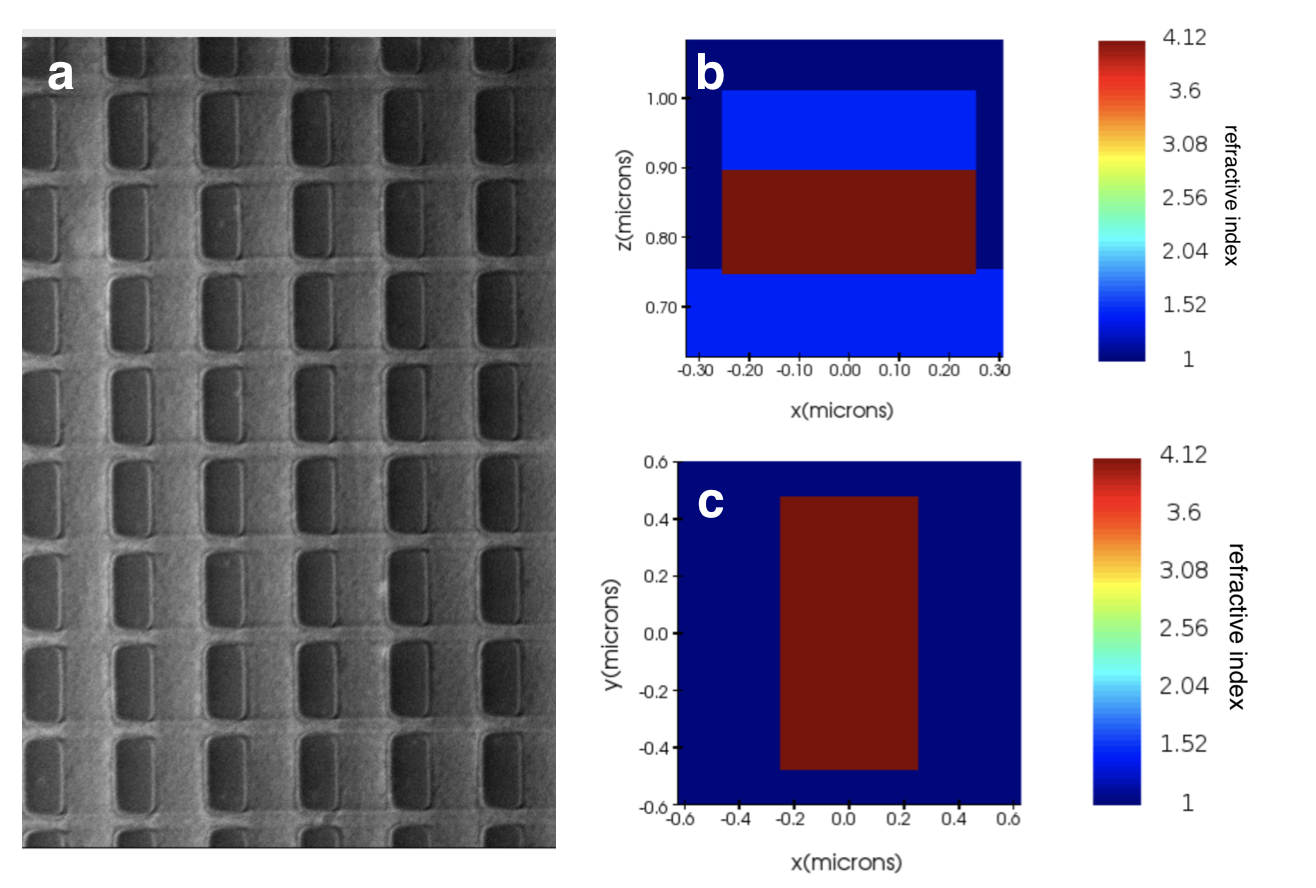
\includegraphics[width=0.8\linewidth]{images/base1.png}
	\caption{На рисунке изображен снимок метаповерхности. В качестве подложки используется $CaF_2$. На подложке с горизонтальным  0,75мкм и с вертикальным шагом 0,25мкм расположенны кирпичики германия (Ge) толщиной 0,15мкм. Наверху каждого кирпичика германия расположен слой  $SiO_2$ толщиной $\sim 0,1$мкм. Изображение на вставке - вид модели с верху, цветная шкала справа показывает показатель преломление структуры}
	\label{base1}
\end{figure}

\subsection{Исследование оптического линейного отклика метаповерхности на основе германия}
\hspace{2mm}
Моделирование отклика структуры производилось в программе lumericl. Периодическая структура освещаться плоской волной с нулевым углов поляризации. На рисунке\ref{base2} изображен один период метаповерхности. Для экономии памяти и времени моделирования был построен только один период поверхности, на границах которого были реализованные граничные периодические условия. Также, для экономии процессорного времени была использована симметрия поверхности: видно, что кирпичик германия симметричен относительно осей OX и OY. Поэтому программа производила расчеты только по 1/4 части  периода поверхности, а затем симметрично отображала полученный результат на остальные 3 области, в которых распределение полей симметрично первой области (в следсвии симметрии, описанной выше).  Монитор a1 (рис.  \ref{base2}а) расположен выше источника электромагнитных волн и измеряет отражение структуры (рис. \ref{1:wave_eq}c), а монитор a2 (рис. \ref{base2}а) расположен ниже кирпичика германия и измеряет пропускание структуры (рис. \ref{base2}b). 
\\
В следствии моделирование были получены графики \ref{base2}b, c, d. На \ref{base2}b можно наблюдать распределение полей в ячейке при резонансе. Черный контур на рисунке соответствует границам кирпичика германия. Свет локализуется внутри элементарной ячейки метаповерхности как показано на рис. \ref{base2}b, приводя к образованию узкого резонанса. Видно, что поле внутри кирпичика германия имеет две симметричные точки одинаковой интенсивности Резонанс также можно наблюдать как в спектре пропускания (рис. \ref{base2}с) так и в спектре отражения структуры (рис \ref{base2}с).  Из графиков видно, что резонанс достигаться на длине волны  $\lambda \approx 2$мкм. Наблюдаемый резонанс возникает из-за геометрических особенностей метаповерхности. 
\begin{figure}[h]
	\centering
    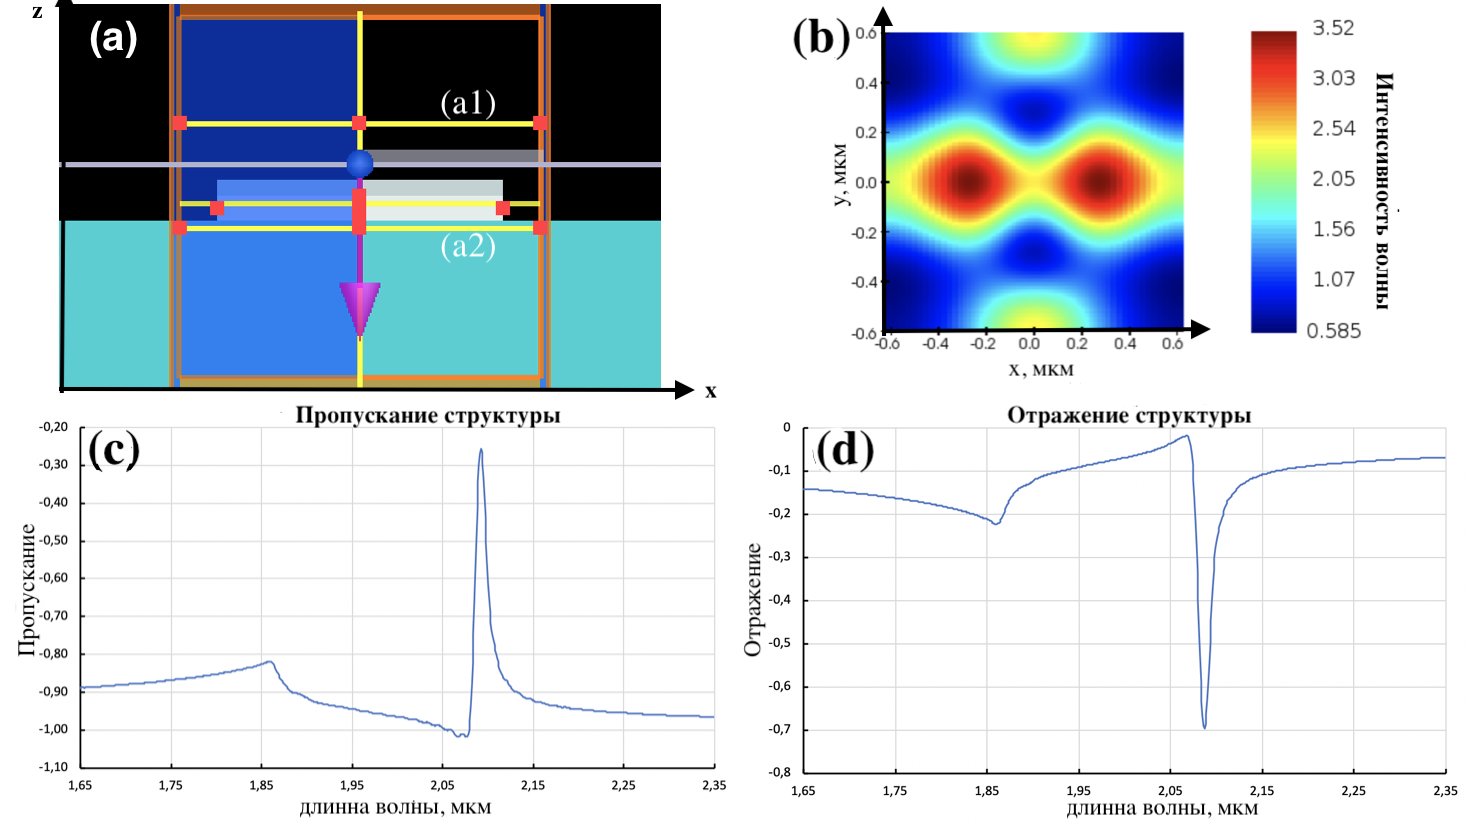
\includegraphics[width=0.9\linewidth]{images/expert.png}
	\caption{\textbf{(a)}На рисунке изображен 1 период метаповерхности, а также мониторы:  \textbf{"а1"}, меряющий отражение структуры, \textbf{"а2"} - меряющий пропускание структуры.  На \textbf{(b)} показано распределение электрического поля в германии во время резонанса. На графиках \textbf{ (c, d)} представлены показания этих мониторов. Резонанс достигаться при длине волны накачки $\lambda = 2,085$мкм.}
	\label{base2}
\end{figure}


